\chapter{Clasificación con Deep Learning}\label{cap.clasificacion}
En este capítulo se expondrá el trabajo realizado para el entendimiento del problema de clasificación, mediante la elaboración de un componente en Python que permite la clasificación de dígitos del 0 al 9 en tiempo real, y la realización de un amplio estudio sobre las variantes posibles aplicadas a las redes entrenadas, utilizando la plataforma Caffe.\\
\section{Clasificador de dígitos}
Se ha desarrollado un componente en Pyhton para la clasificación de dígitos entre 0 y 9 en tiempo real, siendo necesario, previamente, un entendimiento de una primera red básica, utilizada por el mismo para la tarea. En esta sección se explicará el procedimiento seguido para el entendimiento de la red y el desarrollo del propio componente.\\
\subsection{Red básica}\label{sec.red}
La red que se empleará, está orientada a la clasificación de números utilizando, en el entrenamiento, la base de datos numérica MNIST, explicada en la Sección~\ref{sec.minst}.\\
Para realizar el entrenamiento de la red, Caffe proporciona tres archivos que se editarán para adaptar la red al problema que se abarque. A continuación, se explicará cada uno de esos archivos, siguiendo el orden que fue necesario hasta conseguir la red completamente entrenada.
\vspace{15pt}
\subsubsection{Definición de la red}
	Caffe utiliza el archivo 
	\textit{lenet\_train\_test.prototxt} para la especificación de todos los parámetros que son necesarios en el entrenamiento de la red, es decir, define las imágenes que se emplearán, la propia estructura de la red y la forma en la que se analizarán las imágenes proporcionadas, todo ello empleando diferentes capas (\textit{layers}).\\

	La primera línea de este documento es utilizada para indicar el nombre que se le quiere dar a la red.
	\vspace{10pt}
	\begin{lstlisting}[frame=single]
	name: "LeNet"
	\end{lstlisting}
	
	En concreto, esta red recibe el nombre de LeNet, un tipo de red que es conocida por un buen funcionamiento en las tareas de clasificiación de dígitos y que, por lo general, consta de una capa convolucional seguida por una capa de agrupamiento (\textit{pooling}), repetido dos veces y, finalmente, dos capas totalmente conectadas similares a las perceptrones multicapa convencionales. En el ejemplo de Caffe, la estructura habitual de la red LeNet se ve ligeramente modificada, ya que en lugar de emplear una función de activacion sigmoidal se utiliza una linear.\\

	Tras la definición del nombre se definen dos capas de datos, una de ellas correspondiente a los datos de entrenamiento de la red y, la otra, correspondiente a los datos que se utilizarán para realizar el test durante el entrenamiento para obtener datos de \textit{accuracy} y \textit{loss}.
	\vspace{10pt}
	\begin{lstlisting}[frame=single]
	layer {
		name: "mnist"
		type: "Data"
		top: "data"
		top: "label"
		include {phase: TRAIN}
		transform_param {scale: 0.00390625}
		data_param {
			source: "examples/mnist/mnist_train_lmdb"
			batch_size: 64
			backend: LMDB
		}
	}
	\end{lstlisting}
	
	Es importante que los parámetros de transformación, en este caso un factor de escala que establece el rango de la imagen en [0,1], sean los mismos en ambas fases, pues si se evaluase la red con una transformación de la imágen distinta a la aplicada en el entrenamiento los resultados obtenidos no serían reales.\\
	Se utilizará, por tanto, dos capas de datos que difieren en la fase en la que se utilizarán los datos, entrenamiento o evaluación de la red, el tamaño del lote, siendo 64 muestras para el entrenamiento y 100 para el test, y la ruta de la que se cogen los datos.\\
	
	El conjunto de datos proporcionado por MNIST no contiene una base de datos de validación, por lo que se debe dividir la base de datos de entrenamiento en dos partes, una de ellas se utilizará para el entrenamiento y la otra para la validación, incluyendola en la capa de datos de test. Para esta tarea, se desarrolla un script, \textit{createvalidationdatabase.py}, que divide la base de datos de entrenamiento original en dos, el 80\% para entrenamiento y el 20\% restante para validación.\\
	
	\begin{table}[htb]
		\centering
		\begin{tabular}{|l|l|l|l|}
			\hline
			Dígito & Total & 80\% & 20\% \\
			\hline \hline
			0 & 5923 & 4738 & 1185\\ \hline
			1 & 6742 & 5393 & 1349\\ \hline
			2 & 5958 & 4767 & 1191\\ \hline
			3 & 6131 & 4905 & 1226\\ \hline
			4 & 5842 & 4674 & 1168\\ \hline
			5 & 5421 & 4337 & 1084\\ \hline
			6 & 5918 & 4734 & 1184\\ \hline
			7 & 6265 & 5012 & 1253\\ \hline
			8 & 5851 & 4681 & 1170\\ \hline
			9 & 5949 & 4759 & 1190\\ \hline
			Total & 60000 & 48000 & 12000\\ \hline
		\end{tabular}
		\caption{División base de datos de entrenamiento}
		\label{tabla:sencilla2}
	\end{table}
	\vspace{20pt}
	En este proceso es muy importante respetar las proporciones existentes en cada dígito para no alterar la naturaleza de la base de datos original.\\
	
	A continuación, se comienzan a definir las capas del entrenamiento propiamente dicho. Se intercala una capa de convolución con una de agrupamiento y se repite dos veces.
	\vspace{10pt}
	\begin{lstlisting}[frame=single]
	layer {
		name: "conv1"
		type: "Convolution"
		bottom: "data"
		top: "conv1"
		param {lr_mult: 1}
		param {lr_mult: 2}
		convolution_param {
			num_output: 20
			kernel_size: 5
			stride: 1
			weight_filler {type: "xavier"}
			bias_filler {type: "constant"}
		}
	}	
	\end{lstlisting}

	En la capa de convolución, explicada en la Sección~\ref{sec.caffe}, se define que el tamaño del filtro será de 5x5 y que se obtendrán 20 salidas, en la segunda capa de convolución, sin embargo, se obtendrán 50 salidas. Además se define el algoritmo "Xavier" para la inicialización de los pesos, que determina automáticamente la escala de inicialización basada en el número de entradas y de las neuronas de salida, y la inicialización del \textit{bias} mediante una constante que por defecto es 0.
	\vspace{10pt}
	\begin{lstlisting}[frame=single]
	layer {
		name: "pool1"
		type: "Pooling"
		bottom: "conv1"
		top: "pool1"
		pooling_param {
			pool: MAX
			kernel_size: 2
			stride: 2
		}
	}	
	\end{lstlisting}
	
	La capa de agrupamiento, también explicada en la Sección~\ref{sec.caffe}, será alimentada por la capa de convolución anterior y alimentará a la siguiente en caso de que la haya. Se definen en ella un tamaño de filtro de 2x2, un intervalo de dos muestras entre cada aplicación del filtro, por lo que no hay solape, y el método del máximo para realizar el agrupamiento.\\

	Tras estas capas, se establecen dos capas completamente conectadas, \textit{InnerProduct}, separadas por la capa de activación, \textit{ReLu}, ambas explicadas en la Sección~\ref{sec.caffe}. 
	\vspace{10pt}
	\begin{lstlisting}[frame=single]
	layer {
		name: "ip1"
		type: "InnerProduct"
		bottom: "pool2"
		top: "ip1"
		param {lr_mult: 1}
		param {lr_mult: 2}
		inner_product_param {
			num_output: 500
			weight_filler {type: "xavier"}
			bias_filler {type: "constant"}
		}
	}	
	\end{lstlisting}
	
	\begin{lstlisting}[frame=single]
	layer {
		name: "relu1"
		type: "ReLU"
		bottom: "ip1"
		top: "ip1"
	}	
	\end{lstlisting}
	
	Las capas completamente conectadas se definen con, 500 salidas la primera de ellas, y tantas como clases se tengan en la segunda, en el caso concreto que se trata serán 10, correspondientes con los dígitos del 0 al 9.\\

	Para terminar la estructura de la red básica, Caffe permite la opción de añadir capas que muestren parámetros de evaluación de la red que se está entrenando. Para ello, en la Sección~\ref{sec.caffe}, se explicaron varias capas de \textit{Loss}, que serán empleadas en esta red para su evaluación, se deberán explicitar en este documento.
	\vspace{10pt}
	\begin{lstlisting}[frame=single]
	layer {
		name: "accuracy"
		type: "Accuracy"
		bottom: "ip2"
		bottom: "label"
		top: "accuracy"
		include {phase: TEST}
	}
	
	layer {
		name: "loss"
		type: "SoftmaxWithLoss"
		bottom: "ip2"
		bottom: "label"
		top: "loss"
	}	
	\end{lstlisting}
	
	Estas dos capas permiten obtener valores de precisión y pérdidas cada ciertas iteraciones, siendo marcado este valor en el siguiente documento.\\

	En la Figura~\ref{fig.redBasica} se puede observar un esquema de la estructura definida en este apartado, los valores de interés y cada una de las entradas y salidas de las capas. Para obtener esta figura, se ha ejecutado un código proporcionado por la propia plataforma, que, mediante el archivo que define la estructura, explicado anteriormente, dibuja la red. Para ello se debe ejecutar el siguiente comando:
	\vspace{10pt}
	\begin{lstlisting}[frame=single]
	$ caffe/python/draw_net.py <netprototxt_filename> <out_img_filename>
	\end{lstlisting}
	
	\begin{figure}[H]
		\begin{center}
			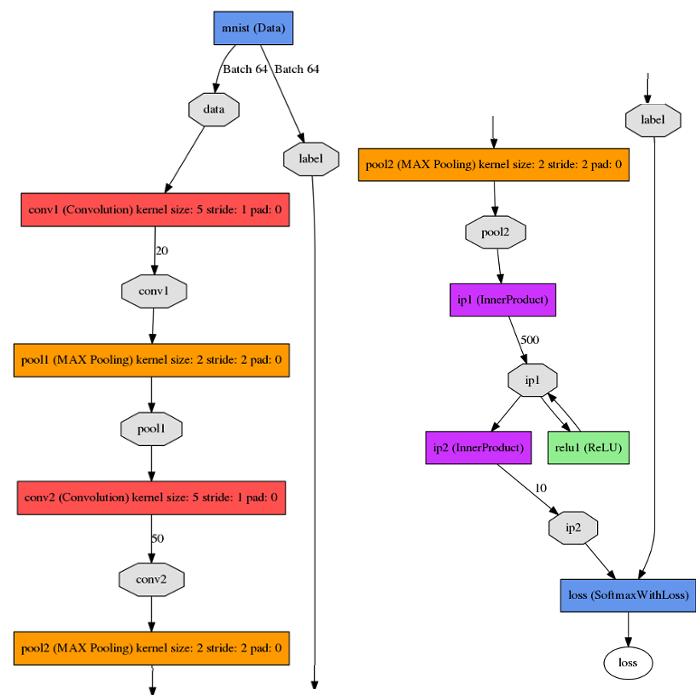
\includegraphics[width=0.8\textwidth]{figures/Original_net}
			\caption{Red básica LeNet MNIST}
			\label{fig.redBasica}
		\end{center}
	\end{figure}
	
\subsubsection{Definición del solucionador}
	Para esta tarea se va a utilizar el archivo de Caffe \textit{lenet\_solver.prototxt}, que permitirá manejar parámetros del propio entrenamiento de la red.\\ 
	Se definen en él parámetros como la estructura de red que se utilizará, definida en el apartado anterior, y el número de iteraciones que se ejecutarán durante el entrenamiento de la red, cuya explicación se aportó en la Sección~\ref{sec.caffe}. Además, en ese mismo capítulo, se explican el resto de parámetros que se manejarán en este proyecto, como la evaluación de la red o las redes intermedias que se guardarán.
	\vspace{10pt}
	\begin{lstlisting}[frame=single]
	# The train/test net protocol buffer definition
	net: "examples/mnist/lenet_train_test.prototxt"
	# test_iter specifies how many forward passes the test should carry 
	# out.
	# In the case of MNIST, we have test batch size 100 and 100 test
	# iterations, covering the full 10,000 testing images.
	test_iter: 100
	# Carry out testing every 500 training iterations.
	test_interval: 500
	# The base learning rate, momentum and the weight decay of the network.
	base_lr: 0.01
	momentum: 0.9
	weight_decay: 0.0005
	# The learning rate policy
	lr_policy: "inv"
	gamma: 0.0001
	power: 0.75
	# Display every 100 iterations
	display: 100
	# The maximum number of iterations
	max_iter: 10000
	# snapshot intermediate results
	snapshot: 5000
	snapshot_prefix: "examples/mnist/lenet"
	# solver mode: CPU or GPU
	solver_mode: CPU	
	\end{lstlisting}
\subsubsection{Ejecución de la red}
	Una vez se han definido los parámetros adecuados para la red que se quiera entrenar, se ejecutarán los siguientes comandos, que comenzará con el entrenamiento de la red:
	\vspace{10pt}
	\begin{lstlisting}[frame=single]
	cd $CAFFE_ROOT
	./examples/mnist/train_lenet.sh	
	\end{lstlisting}
	
	El archivo que se ejecuta contiene información sobre qué solucionador se debe implementar y el modo de ejecución. Además es posible añadirle una línea que guardará un archivo con información de \textit{log} del proceso de entrenamiento.
	\vspace{10pt}
	\begin{lstlisting}[frame=single]
	#!/usr/bin/env sh
	set -e
	
	./build/tools/caffe train 
	  --solver=examples/mnist/lenet_solver_validation.prototxt 
	    2>&1 | tee /home/nuria/TFG/logs/RedBasica.log $@
	\end{lstlisting}
	
	\begin{figure}[H]
		\begin{center}
			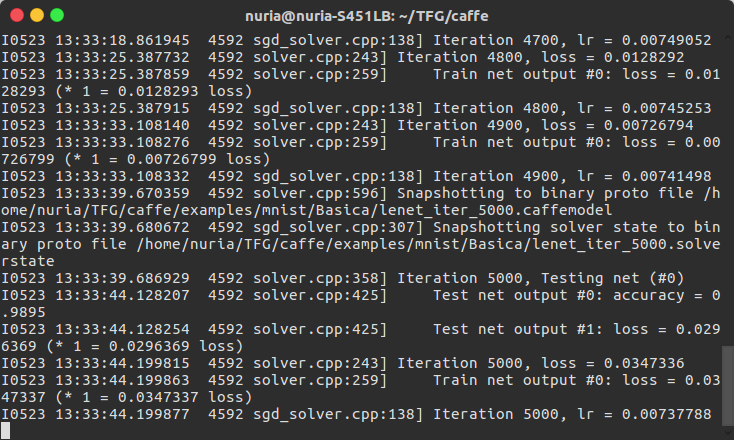
\includegraphics[width=0.8\textwidth]{figures/RedBasica5000}
			\caption{Ejecución de entrenamiento de red LeNet MNIST}
		\end{center}
	\end{figure}
	
	\begin{figure}[H]
		\begin{center}
			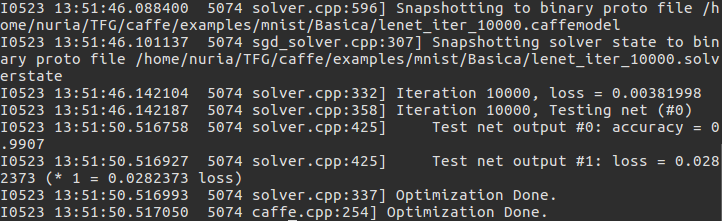
\includegraphics[width=0.8\textwidth]{figures/RedBasicaFin}
			\caption{Fin de entrenamiento de red LeNet MNIST}
			\label{fig.finEntrBas}
		\end{center}
	\end{figure}
	
	Tras terminar el entrenamiento, mostrado en la Figura~\ref{fig.finEntrBas}, se obtiene el archivo con la red neuronal entrenada, almacenado según la ruta que se indicó en el solucionador, que podrá ser utilizada en la herramienta que sea de interés.\\

	El archivo \textit{log} generado podrá ser visualizado mediante la ejecución del script \textit{plot\_learning\_curve.py} \footnote{https://github.com/adilmoujahid/deeplearning-cats-dogs-tutorial/blob/master/code/plot\_learning\_curve.py} de la siguiente forma:
	\vspace{10pt}
	\begin{lstlisting}[frame=single]
	python plot_learning_curve.py /home/nuria/TFG/logs/RedBasica.log 
	 RedBasicaLog.png
	\end{lstlisting}
	
	En la Figura~\ref{fig.Log} se puede observar el resultado final de la curva de aprendizaje, con valores de precisión y pérdidas, según lo explicado en la Sección~\ref{sec.caffe}, para la fase de evaluación, y en entrenamiento únicamente de pérdidas.
	
	\begin{figure}[H]
		\begin{center}
			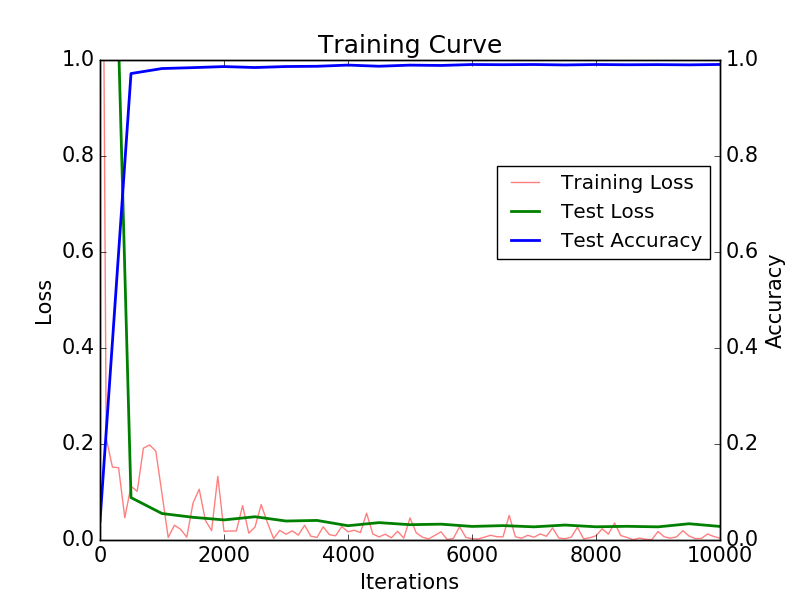
\includegraphics[width=0.5\textwidth]{figures/RedBasicaLog}
			\caption{Curva de aprendizaje Red Básica}
			\label{fig.Log}
		\end{center}
	\end{figure}

\subsection{Componente Python}
Se ha desarrollado un componente escrito en Python que, mediante la ayuda del \textit{Camera Server} de JdeRobot, comentado en la Sección~\ref{sec.jderobot},  y la red explicada en la Sección~\ref{sec.red}, es capaz de clasificar un dígito mostrado a la cámara, que se especificará en un archivo de configuración, en tiempo real, encendiendo una bombilla que se corresponde con el número obtenido.\\

Debido a la magnitud de la tarea a realizar, se optó por dividir el programa en dos hilos que serán explicados a continuación. Uno de ellos se encargará del aspecto gráfico de la aplicación, mostrando la imagen obtenida por la cámara, la imagen procesada para la clasificación, y la iluminación de la bombilla correspondiente. El segundo hilo, se encargará de gestionar la captación de la cámara, mediante la conexión con el componente \textit{Camera Server}, así como el proceso de clasificación, utilizando la red entrenada. Todo el código correspondiente a esta aplicación podrá ser encontrado en 
\subsubsection{Cámara} \label{sec.camara}
El hilo fundamental de la aplicación, que se encargará de la lógica de la misma mediante la adquisición de la imagen y su posterior procesamiento, estará referenciado por el nombre \textit{Camera}.\\

Al comienzo de la ejecución se inicializa un objeto Cámara, mediante el constructor \textit{Camera()}, que será el encargado de gestionar las acciones anteriormente nombradas. En esta inicialización se indica qué cámara se va a utilizar, referenciada de manera externa mediante un archivo de configuración que se indicará en la ejecución de la aplicación. La línea que indica la cámara en este archivo es la siguiente:
\vspace{10pt}
\begin{lstlisting}[frame=single]
	Numberclassifier.Camera.Proxy=cameraA:default -h localhost -p 9999
\end{lstlisting}
Esta propiedad estará enlazada con el componente \textit{Camera Server} de JdeRobot que nos proporciona un servidor de imágenes mediante la cámara.\\

Otro aspecto importante que se maneja en la inicialización de la cámara es la especificación y carga de la red que se empleará para la clasificación. Este aspecto se realiza mediante las siguientes líneas:
\vspace{10pt}
\begin{lstlisting}[frame=single]
	model_file = '/home/nuria/TFG/caffe/examples/mnist/lenet.prototxt'
	pretrained_file = '/home/nuria/TFG/caffe/examples/mnist/Basica/
						/lenet_iter_10000.solverstate'
	self.net = caffe.Classifier(model_file, pretrained_file, 
									image_dims=(28, 28), raw_scale=255)
\end{lstlisting}
Mediante estas líneas se realizan las tres acciones necesarias para establecer la red que se utilizará. En primer lugar, se indica cuál será el modelo empleado para la clasificación. Este modelo es un archivo porporcionado Caffe de manera homóloga al \textit{lenet\_train\_test.prototxt}, con la excepción de que la capa de datos no recurre a archivos almacenados sino que utiliza imágenes que serán insertadas en la ejecución de la red. El resto de datos deben ser exáctamente iguales a la estructura de la red entrenada para que no se produzcan errores. En segundo lugar, se indica la red entrenada que se utilizará en la ejecución, el archivo obtenido al finalizar el entrenamiento según se indicó en la Sección~\ref{sec.red}. Por último, se crea la red ejecutable, es decir, se crea un objeto que será utilizado por la aplicación cada vez que se quiera realizar la clasificación. Para esta creación es necesario indicar, en primer lugar, que se trata de una red para la clasificación, y, además, introducir los parámetros del modelo, la red entrenada, las dimensiones de las imágenes, y la escala de los píxeles.\\

Además de las propiedades más importantes comentadas anteriormente, se definen también, funciones que serán importantes para la ejecución de la aplicación. Se establece una función \textit{update(self)}, que será llamada cada 150ms ya que, en el componente principal, se crea el hilo \textit{ThreadCamera(camera)} para obtener las imágenes de forma periódica y poder establecer un flujo de vídeo a tiempo real. Esta función, a su vez, necesita de otra, \textit{getImage(self)}, que obtiene la imagen, la redimensiona, y le aplica una transformación necesaria antes de introducirla en el proceso de clasificación, devolviendo un array con las dos imágenes, original y transformada. Para esa transformación se utiliza una tercera función de la cámara, \textit{trasformImage(self,img)}. En ella, se centra la imagen en un cuadrado, pues la captada es rectangular y la necesaria para introducir en la red cuadrada, se convierte a imagen de grises, se redimensiona al tamaño necesario para introducirla en la red (28x28), y por último, se le aplica un filtro gaussiano de 5x5 para reducir el ruido.\\

Finalmente, se crea una función para realizar la clasificación de los dígitos:
\vspace{10pt}
\begin{lstlisting}[frame=single]
	def classification(self, img):
		self.net.blobs['data'].reshape(1,1,28,28)
		self.net.blobs['data'].data[...]=img * 0.00390625
		output = self.net.forward()
		digito = output['prob'].argmax()
		return digito
\end{lstlisting}
En primer lugar se asegura que las dimensiones del \textit{bolb} de datos sea de 28x28, valores establecidos para las imágenes. En el siguiente paso, se introduce a la red la imagen obtenida tras la transformación, aplicandole el factor de escala para que el intervalo de los píxeles esté entre 0 y 1, pues eso fue lo que se indicó en el aprendizaje. Posteriormente se ejecuta la red y se obtiene, como salida, una estructura que almacena, por un lado, la propiedad \textit{'prob'}, que se corresponde con un array que incluye las probabilidades de que la imagen introducida sea cada uno de los dígitos posibles, y, por otro, el tipo de datos que se almacena, en este caso \textit{float32}. Posteriormente, de ese array de probabilidades, se escoge el dígito cuya probabilidad es mayor, es decir, la clasificación realizada, y se devuelve.\\

Una vez establecida la lógica de la aplicación, se pasa a desarrollar el interfaz gráfico que permite al usuario visualizar, tanto las imágenes captadas y transformadas, como el resultado de la clasificación.
\subsubsection{GUI}
Para el aspecto gráfico de la aplicación, en el componente principal, se inicializará un objeto llamado \textit{window} mediante el constructor \textit{Gui()}, al que posteriormente se le vinculará la cámara mediante una función propia, \textit{window.setCamera(camera)}. Por último, al tratarse de un componente gráfico, será necesario indicar que se muestre mediante \textit{window.show()}. Al inicializar este objeto se crean todos los elementos gráficos que serán necesarios y que se modificarán posteriormente para conseguir el resultado deseado.\\

Al igual que en el caso de la cámara, se estabelcerá un hilo que permita aligerar la ejecución de la aplicación mediante \textit{ThreadGui(window)}, que establece el tiempo de actualización en 50ms. Debido al uso de este hilo, se crea en el objeto una función \textit{update()} que, en este caso, se encarga de obtener las imágenes original y transformada mediante la función \textit{getImage()} de la cámara, y adaptarlas para poder mostrarlas en las etiquetas definidas para cada una de ellas. Además, llama a otra función propia, \textit{lightON(out)}, que cambia el color del fondo del dígito que se haya clasificado, haciendo uso de la función de clasificación definida anteriormente en la cámara.\\

En la Figura~\ref{fig.gui} se puede observar el resultado gráfico de la aplicación. Al no tener detección, la ejecución de la clasificación es continua, por lo que, aunque no exista un dígito en la imagen, el componente decide constantemente un determinado dígito que considerará correcto, encendiendo la bombilla adecuada.\\

\begin{figure}[H]
	\begin{center}
		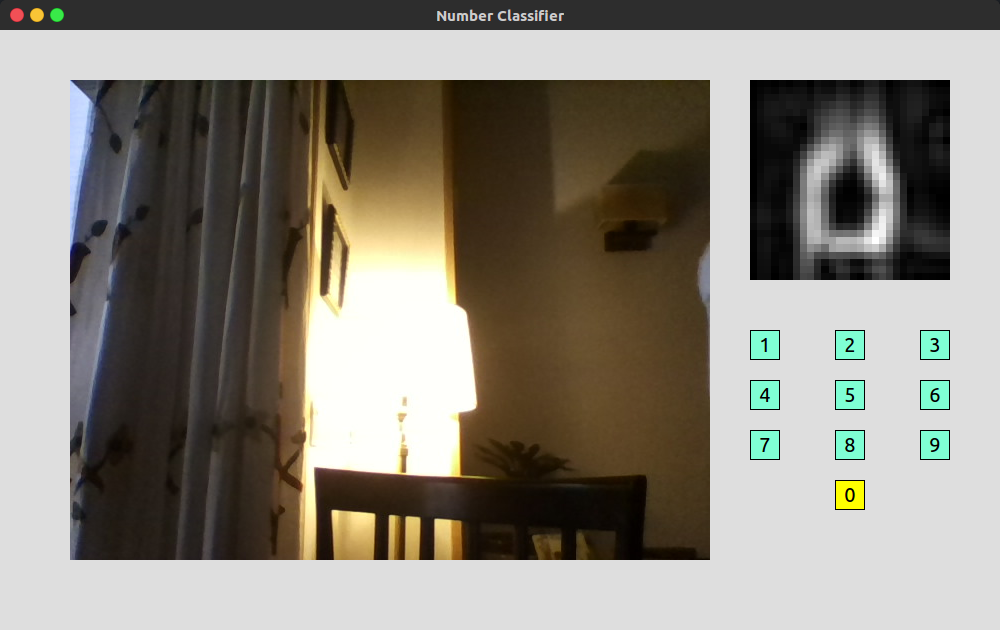
\includegraphics[width=0.8\textwidth]{figures/gui}
		\caption{Captura de componente gráfico de la aplicación}
		\label{fig.gui}
	\end{center}
\end{figure}

\subsubsection{Ejecución}
El proceso de ejecución del componente se divide en dos pasos. Por un lado, será necesaria la ejecución del servidor de imágenes, para lo que se utilizará el componente de JdeRobot. Por otro lado se debe lanzar el propio componente clasificador explicado anteriormente.\\

Para ejecutar el \textit{Camera Server}, se seguirán las instrucciones que aporta la plartaforma JdeRobot, utilizando el archivo de configuración que se facilita. Se utilizará el siguiente comando: 
\vspace{10pt}
\begin{lstlisting}[frame=single]
	cameraserver cameraserver.cfg
\end{lstlisting}

En el desarrollo de este trabajo, la propiedad de interés del archivo de configuración es \textit{CameraSrv.Camera.0.Uri}, que se centra en indicar la fuente de vídeo. Esta fuente puede ser un archivo de vídeo almacenado, para el que se emplearía la ruta del archivo en ese campo, la webcam del propio ordenador, para el que se utilizará el valor 0, u otra cámara externa, para la que se indicará el valor 1.\\

En la Sección~\ref{sec.droid} se comentó una aplicación que permitía utilizar la camara de un smartphone android como fuente de vídeo mediante una cámara externa. Para poder utilizar esta herramienta es necesario tener instalada el programa tanto en el dispositivo móvil a utilizar como en el propio ordenador, según se indica en las guía de la aplicación \footnote{https://www.dev47apps.com/droidcam/linuxx/}, y abrir la aplicación. Una vez abierta en ambos dispositivos, se debe conectar el USB del ordenador al móvil e indicar en la aplicación de escritorio que la conexión se hará vía USB. Se opta por la conexión USB, pues es más rápida y, por tanto, más adecuada a tiempo real. Una vez se han realizado las acciones anteriores se estable la conexión y se obtienen los resultados de las Figuras~\ref{fig.droidEsc}, en el ordenador, y ~\ref{fig.droidMov}, en el dispositivo.\\

\begin{figure}[H]
	\begin{center}
		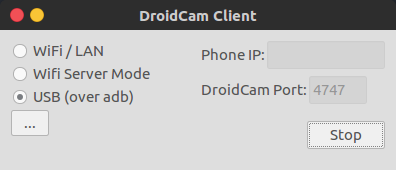
\includegraphics[width=0.4\textwidth]{figures/droidcamEscr}
		\caption{Captura de DroidCam en el ordenador}
		\label{fig.droidEsc}
	\end{center}
\end{figure}

\begin{figure}[H]
	\begin{center}
		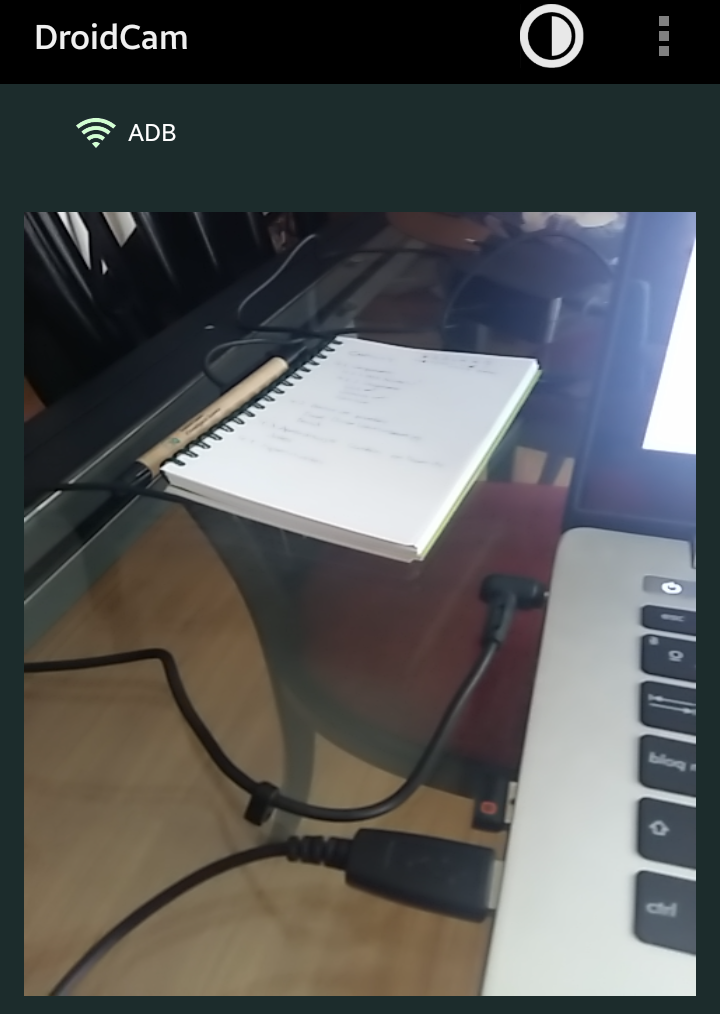
\includegraphics[width=0.3\textwidth]{figures/droidcamMov}
		\caption{Captura de DroidCam\\ 
			en el dispositivo móvil}
		\label{fig.droidMov}
	\end{center}
\end{figure}

Tras tener en funcionamiento el servidor de imágenes se debe proceder a la ejecución del componente clasificador. Para ello se ejecutará el siguiente comando:
\vspace{10pt}
\begin{lstlisting}[frame=single]
	python numberclassifier.py --Ice.Config=numberclassifier.cfg
\end{lstlisting}

El componente Python contiene los procedimientos indicados en las secciones anteriores, la creación del GUI, la cámara y el lanzamiento de los hilos correspondiente a cada uno. En el fichero de configuración se tiene una porpiedad que indica qué cámara utilizar. Es importante que el nombre de esta cámara se corresponda con el indicado en el fichero de configuración del servidor, de esta manera se establece la comunicación entre ambos componentes.\\

Finalmente, tras la ejecución, obtenemos el resultado del componente mostrado en la Figura~\ref{fig.componente1}, donde se aprecia el funcionamiento del mismo para un número sencillo y perfectamente definido según el entrenamiento de la red, es decir, fondo negro y número blanco.\\

Tras conseguir la aplicación del clasificador, se ha evaluado la red obtenida mediante un banco de pruebas, que será explicado a continuación y se ha procedido a la mejora de la misma.

\begin{figure}[H]
	\begin{center}
		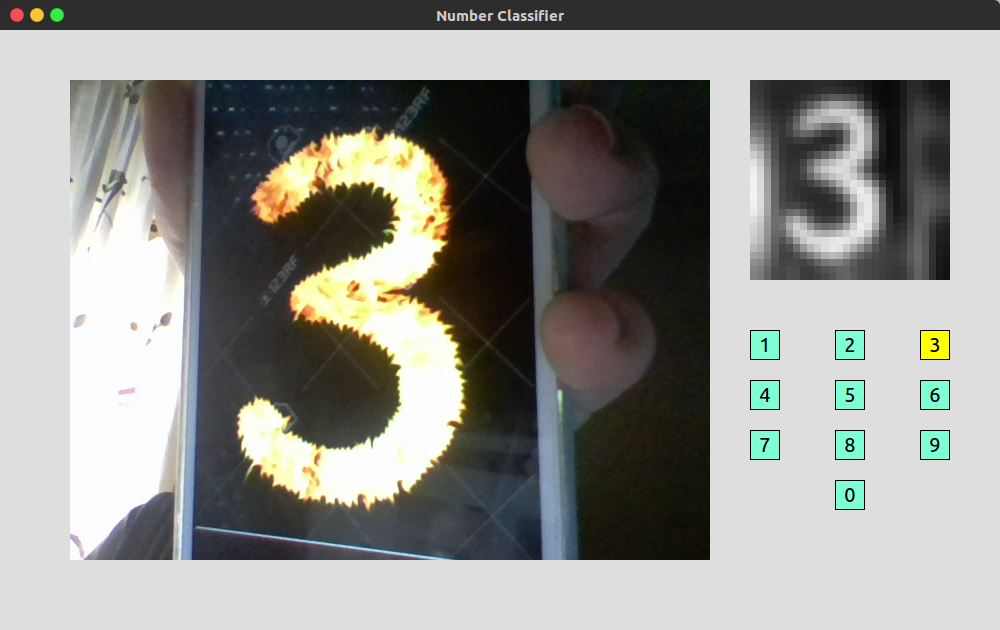
\includegraphics[width=0.5\textwidth]{figures/componente1}
		\caption{Captura del componente clasificador}
		\label{fig.componente1}
	\end{center}
\end{figure}
\vspace{30pt}
\section{Banco de pruebas} \label{sec.banco}
Para la evaluación de las diferentes redes neuronales que se desarrollarán en el proyecto se elabora un banco de pruebas que permite obtener las métricas explicadas en el Capítulo~\ref{cap.infraestructura}, siendo necesario, previamente, la obtención de datos de clasifciación sobre una determinada base de datos de evaluación.\\
\subsection{Obtención de datos de test}
El primer paso para la elaboración de este banco de pruebas pasa por el desarrollo de un script, \textit{testcaffenet.py}, que permite introducir una base de datos de evaluación a la red neuronal deseada y obtener la clasificación para cada uno de los elementos de esa base de datos. Este script está dividido en tres partes claramente diferenciadas que permite la obtención de los resultados.\\

\begin{description}
	\item[Obtención de las imágenes] \hfill 
	\vspace{10pt}
	\\
	Las imágenes y sus correpondientes etiquetas estan almacenadas en bases de datos de tipo \textit{lmdb}. Este tipo de bases de datos requiere de un método específico para poder acceder al contenido de las mismas y poder manipular las imágenes que se almacenan en ellas.
	\vspace{15pt}
	\begin{lstlisting}[frame=single]
		lmdb_env = lmdb.open('/home/nuria/TFG/lmdb_test/test_lmdb')
		lmdb_txn = lmdb_env.begin()
		lmdb_cursor = lmdb_txn.cursor()
	\end{lstlisting}
	Tras este código, se obtiene un cursor que apunta al comienzo de los datos en la misma y que permitirá recorrerla para obtener las imágenes y etiquetas.\\
	\vspace{-10pt}
	
	Para poder procesar los datos obtenidos mediante Caffe, será necesario crearse una estructura \textit{Datum} de Caffe, que incluirá, en cada iteración para recorrer la base de datos, la información de la instancia de la base de datos. El siguiente código, crea la estructura indicada e indica la forma en que se recorre la base de datos, obteniendo, por un lado, los datos de la imagen en sí (\textit{data}), y por otro, las etiquetas de las mismas (\textit{label}).
	\vspace{10pt}
	\begin{lstlisting}[frame=single]
		datum = caffe.proto.caffe_pb2.Datum()
		...
		for key, value in lmdb_cursor:
			datum.ParseFromString(value)
			label = datum.label
			data = caffe.io.datum_to_array(datum)
			...
	\end{lstlisting}
	Finalmente, en la variable \textit{data} se almacena la imágen que se utilizará posteriormente para realizar la clasificación, y en \textit{label}, la etiqueta correspondiente que se empleará para hacer las comparaciones.
	\vspace{15pt}

	\item[Clasificación de las imágenes] \hfill 
	\vspace{10pt}
	\\
	La tarea de clasificación se realizará exáctamente de la misma manera que se especificó en la Sección~\ref{sec.camara}, utilizando la misma función sobre cada uno de los \textit{data} obtenidos.
	\vspace{10pt}
	\begin{lstlisting}[frame=single]
		...
		net_out = classification(data)
		...
	\end{lstlisting}
	Una vez se ha conseguido obtener el dígito que la red interpreta, se procede a las comparaciones para poder obtener datos más cómodos para la evaluación.
	\vspace{15pt}
	
	\item[Comparación de datos] \hfill 
	\vspace{10pt}
	\\
	La tarea de comparación de los datos obtenidos por la red con los reales almacenados en la base de datos es bastante sencilla. \\
	\vspace{-10pt}
		
	Se ha optado por la creación de un archivo de texto que incluirá una pequeña descripción de cómo interpretar el contenido y, para cada iteración, el número de iteración, las etiquetas reales, las identificadas porla red y un booleano que indicará si ambas etiquetas coinciden o no, todo ello separado por espacios.
	\vspace{10pt}
	\begin{lstlisting}[frame=single]
	for key, value in lmdb_cursor:
		...
		if label == net_out:
			conclusion = True
		else:
			conclusion = False
		testfile.write("Interacion " + str(loop) + ":")
		testfile.write(str(label) + " " + str(net_out) + " " )
		testfile.write(str(conclusion) + "\n")
		loop = loop + 1
		...
	\end{lstlisting}
	Esta estructura permitirá un manejo más cómodo de los datos por el banco de pruebas creado además de un fácil entendimiento para el usuario que lea el archivo de lo que se está mostrando en él.\\
\end{description}
Una vez se ha obtenido el archivo con los datos necesarios para obtener valores que ilustren sobre la robustez de la red, se procede a abarcar la manera en que se procesarán los mismos, obteniendo el banco de pruebas.

\subsection{Banco de pruebas manual: Excel}
Las métricas que se obtienen con este banco de pruebas son las explicadas en la Sección~\ref{sec.metricas}: Matriz de confusión, \textit{precision} y \textit{recall}. De manera externa al banco de pruebas, y gracias a Caffe, se obtendrán también valores de \textit{accuracy}, homólogo a \textit{precision}, y \textit{loss}, para cada uno de las redes intermedias que se obtienen durante el entrenamiento de la red final.\\

Para la elaboración de este banco de pruebas se ha optado por la herramienta de Libre Office Calc, homóloga a Excel, que permite realizar diversas operaciones sobre hojas de cálculo gracias a múltiples fórmulas y funciones. Se han volcado los datos obtenidos con el script anterior estableciendo como separador el espacio y los dos puntos, obteniendo, así, distintas columnas. De estas columnas formadas serán de interés la que contiene la etiqueta real, la clasificación realizada, y la conclusión final, acierto o fallo.\\

Tras obtener los datos de interés separados y correctamente ordenados se procederá a identificar el número de aciertos y de fallos tanto a nivel global, para obtener los parámetros de precisión total o \textit{accuracy}, como a nivel de dígito para obtener la matriz de confusión y con ella los valores de \textit{precision} y \textit{recall} para cada uno de los dígitos.\\

\begin{description}
	\item[Precisión total] \hfill 
	\vspace{10pt}
	\\
	Este valor es el más lógico y sencillo de obtener. Para calcular la precisión total, es decir, la tasa de acierto independientemente del dígito que se trate, basta con contar el número de veces que se ha obtenido el valor \textit{True} en la columna de conclusión y dividirlo entre el número de imágenes de evaluación que se han utilizado para la misma. De esta manera se obtiene el porcentaje de imágenes que se han clasificado de forma correcta, valor que se corresponde con la precisión de la red.\\
	\vspace{-10pt}
	\\
	Para realizar esta operación, el código empleado ha sido dividido en cuatro partes diferenciadas:\\
	\vspace{-20pt}
	\begin{itemize}
		\item{Para obtener el número de clasificaciones correctas:
		\vspace{10pt}
		\begin{lstlisting}[frame=single]
			CONTAR.SI('Sobel sin trasform'.E3:E20002;"True")
		\end{lstlisting}
		Donde:
		\begin{itemize}
			\item 'Sobel sin transform' es la hoja en la que se han volcado los resultados del archivo de texto.
			\item E3:E20002 es la columna que contiene los datos de la conclusión.
			\item "True" indica que se quiere contar el número de veces en esa columna que aparece ese valor
		\end{itemize}
	}
	\item{Para obtener el número de clasificaciones incorrectas:
		\vspace{10pt}
		\begin{lstlisting}[frame=single]
			CONTAR.SI('Sobel sin trasform'.E3:E20002;"False")
		\end{lstlisting}
		Es equivalente al anterior pero, en este caso, se cuenta el número de veces que se cometió un error en la clasificación.
	}
	\item{Para obtener el número de imágenes de evaluación totales: Será suficiente con realizar la suma de los correctos e incorrectos.
	}
	\item{Para calcular el porcentaje de acierto: Para ello se realizará la división del número de acierto entre el total y multiplicarlo por 100 para obtener el porcentaje.
	}
	\end{itemize}
	\vspace{15pt}
	\item[Matriz de confusión] \hfill 
	\vspace{10pt}
	\\
	Tanto para este apartado, como para los dos posteriores, se ha utilizado la información proporcionada por \cite{metrics}.\\
	\vspace{-10pt}
	\\
	Para elaborar la matriz de confusión se parte de la misma hoja de cálculo con las columnas de etiqueta real, clasificada y conclusión del apartado anterior. En este caso se debe de tener en cuenta, para cada dígito real, tanto el número de veces que se clasifica correctamente, como el número de veces que se equivoca con cada uno de los dígitos restantes.\\
	\vspace{-10pt}
	\\
	Se elabrora una tabla en la que se enfrentan los dígitos reales del 0 al 9 con las predicciones posibles en el mismo rango. En concreto, cada columna representa las veces que se introduce una imagen de cada uno de los dígitos y, cada fila, el número de veces que se predice uno de los dígitos.\\
	\vspace{20pt}
	\\
	El código de cada celda queda materializado de la siguiente manera:
	\vspace{10pt}
	\begin{lstlisting}[frame=single]
		CONTAR.SI.CONJUNTO(C3:C70002;"1";D3:D70002;"2")
	\end{lstlisting}
	Donde:
	\begin{itemize}
		\item C3:CC70002 se corresponde con la columna que contiene las etiquetas reales
		\item D3:D70002 se corresponde con la columna que contiene las etiquetas predichas.
		\item Los valores entre comillas, "1" y "2" se corresponde con el dígito en cuestión que se quiera analizar. En este caso, se está contando el número de veces que se ha producido un 1 y se ha predicho, erróneamente, un 2.
	\end{itemize}
	
	De esta forma, cada vez que se prediga un dígito determinado, se sumará uno en la celda que se corresponda con el dígito real introducido en la red y la etiqueta resultante de la predicción.\\
	\vspace{-10pt}
	\\
	Una vez se ha obtenido esta matriz, obtener los valores de \textit{precision} y \textit{recall} resulta bastante sencillo.
	\vspace{15pt}
	\item[\textit{Precision}] \hfill 
	\vspace{10pt}
	\\
	Para obtener el valor de \textit{precision} para cada dígito, se divide el número de veces que se ha clasificado correctamente dicho dígito entre el número de veces totales que se predijo el mismo. Para ello, se suman todos los valores por filas, obteniendo el número de predicciones de cada uno de los dígitos, y se divide cada valor de la diagonal, correspondiente con las clasificaciones correctas, entre el valor suma obtenido en la fila correspondiente.
	\vspace{15pt}
	\item[\textit{Recall}] \hfill 
	\vspace{10pt}
	\\
	Para este parámetro, se debe dividir el número de clasificaciones correctas de cada dígito entre el número de veces que se produjo el mismo. En este caso, se sumarán los valores obtenidos por columnas, lo que dará por resultado el número de veces que se introdujo a la red cada uno de los dígitos. Una vez obtenido ese valor, se debe dividir el valor de la diagonal correspondiente, al igual que en el caso anterior, entre el valor obtenido para cada columna.
\end{description}

\section{Efectos del aprendizaje}
Existen numerosos factores que afectan al nivel de robusted de la red en el proceso de entrenamiento de la misma. Elementos como la base de datos, el número de neuronas empleadas, el número de capas o las etapas que se realizan en el entrenamiento \cite{lopez2008redes}, hacen que la red tenga una mayor, mejorando la aplicación deseada.\\

En esta sección se tratará el efecto en el aprendizaje de tres de los factores que se pueden manipular para adaptar la robusted de la red a la aplicación que se vaya a tratar, estos elementos son el cambio en las bases de datos de entrenamiento, el incremento del número de neuronas y el uso o no del \textit{Dropout}.\\

\subsection{Bases de datos}

La base de datos empleada en el primer ejemplo explicado es excesivamente simple y, por lo tanto, no aporta la robusted necesaria para un problema de clasificación real.\\

El primer problema que se encuentra en esta base de datos es que únicamente se dispone de muestras con el fondo negro y el dígito en blanco. Ésto limita bastante la funcionalidad de la aplicación, ya que se pretende clasificar cualquier dígito, independientemente del fondo sobre el que se muestre. Para estudiar el efecto que tiene el cambio de fondo en las imágenes en la red neuronal desarrollada se ha elaborado una base de datos de evaluación ampliada, incluyendo, para cada muestra, su negativo.\\

La obtención de la base de datos se consigue gracias al script \textit{create\_neg\_database.py}. El proceso llevado a cabo en este script parte del tratamiento de bases de datos de tipo \textit{lmdb} explicado en la Sección~\ref{sec.banco}. Se debe abrir la base de datos con las imágenes originales y utilizar los datos de la imagen obtenidos para realizar la transformación deseada. Posteriormente, para almacenar las imágenes transformadas, se debe abrir una nueva base de datos de este tipo, que permita escritura. Esta apertura se realiza con las siguientes líneas:
\vspace{35pt}
\begin{lstlisting}[frame=single]
	new_lmdb_env = lmdb.open('/home/nuria/TFG/lmdb_test/test_edgesCanny_lmdb',
						map_size=int(1e12))
	new_lmdb_txn = new_lmdb_env.begin(write=True)
	new_lmdb_cursor = new_lmdb_txn.cursor()
	new_datum = caffe.proto.caffe_pb2.Datum()
\end{lstlisting}
Se puede observar que el proceso es muy similar al explicado en la Sección~\ref{sec.banco}, incluyendo dos parámetros que permitan la escritura en la base de datos.\\

Posteriormente, dentro del bucle explicado en la misma sección mencionada, se debe almacenar la imagen original en la nueva base de datos, aplicar el negativo a la imagen, realizando la resta de 255 y la propia imagen, y almacenar, también, la transformación. Para insertar imágenes en una nueva base de datos es necesario realizar dos acciones, la inserción en la base de datos y la actualización de la misma.\\

Para realizar la inserción, al finalizar la interpretación de los datos de cada muestra de la base de datos original, se deben incluir las siguientes líneas:
\vspace{10pt}
\begin{lstlisting}[frame=single]
	new_datum = caffe.io.array_to_datum(data,label)
	keystr = '{:0>8d}'.format(item_id)
	new_lmdb_txn.put( keystr, new_datum.SerializeToString() )
\end{lstlisting}
De esta manera se incluye en la posición \textit{keystr}, la imagen y la etiqueta deseada, a partir del puntero que señala las posiciones dentro de la base de datos.\\

Posteriormente, para la actualización de la base de datos, se deben incluir un nuevo código, que guarda los cambios realizados y actualiza la posición del puntero.
\vspace{10pt}
\begin{lstlisting}[frame=single]
	new_lmdb_txn.commit()
	new_lmdb_txn = new_lmdb_env.begin(write=True)
\end{lstlisting}
Estas líneas se incluyen dentro de un condicional que hará que únicamente se escriba en la base de datos cada cierto tiempo, ya que no es necesario realizar estas acciones en todas las inserciones realizadas, ahorrando carga computacional.\\

En la Figura~\ref{fig.neg} se muestra uno de los dígitos y su correspondiente negativo almacenado en la base de datos. Estas imágenes han sido obtenidas con el script \textit{dataread.py}, que lee las imágenes de la base de datos y crea un archivo para su visualización.\\

\begin{figure}[H]
	\begin{center}
		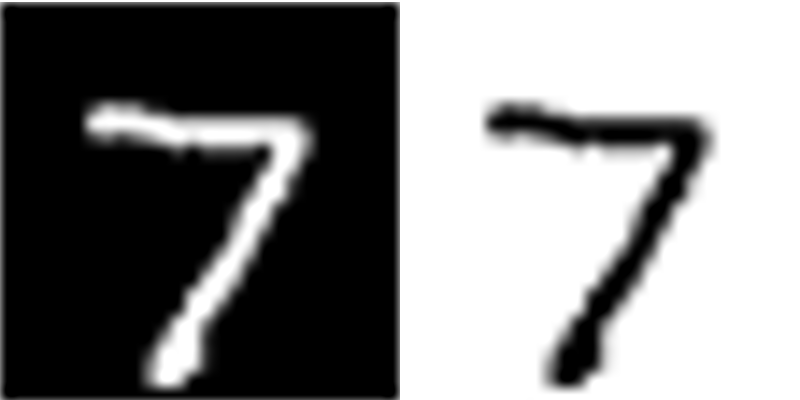
\includegraphics[width=0.5\textwidth]{figures/negativo}
		\caption{Imagen original y su correspondiente negativo}
		\label{fig.neg}
	\end{center}
\end{figure}

Tras ejecutar este script se obtiene la base de datos de evaluación con los negativos, la cual tendrá el doble de muestras que en el caso original, es decir 20000. Ésta es introducida en el banco de pruebas explicado y se obtienen valores de precisión global.\\

En la Figura~\ref{fig.neg-orig} se muestran los resultados obtenidos, donde se puede observar que la red falla consideráblemente al incluir las imágenes en negativo. Se obtiene un porcentaje de acierto cercano al 60\%, lo que se corresponde, en su práctica totalidad, a la clasificación correcta de las imágenes originales.\\

\begin{figure}[H]
	\begin{center}
		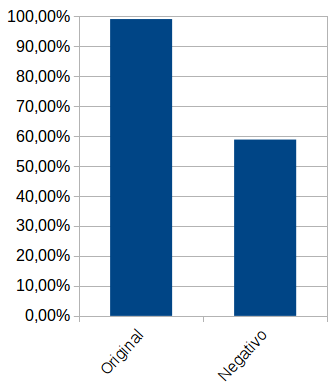
\includegraphics[width=0.5\textwidth]{figures/orig_neg}
		\caption{Porcentaje de acierto de base de datos \\
			original y ampliada con negativo}
		\label{fig.neg-orig}
	\end{center}
\end{figure}

Para solucionar el problema que acarrea el tener esta gran diferencia únicamente modificando el fondo de la imagen, y puesto que la aplicación no está enfocada a un único tipo de fondo, se opta por aplicar un filtro de bordes que independice la imagen del fondo. Existen varios filtros de bordes que es posible aplicar para solucionar el problema, todos ellos se basan en la localización en la imagen de aquellas zonas en las que la diferencia de valor entre un píxel y el contiguo supera un determinado umbral \cite{fundamentos}.\\

Para desarrollar la comparación entre los diferentes filtros posibles se ha desarrollado un script similar al anterior, en el que se aplicaba el negativo, \textit{create\_edges\_database.py}. En este caso, se parte de la base de datos ampliada con el negativo, no siendo necesario almacenar la imagen de la que se parte en la base de datos, y sustituyendo el negativo por el filtro adecuado en la transformación. Además, será necesario aplicar el mismo sobre la base de datos de entrenamiento, puesto que el objetivo es desarrollar una nueva red neuronal que interprete los bordes. Se obtiene, así, una base de datos de entrenamiento con 48000 muestras y, otra de evaluación, con 20000 muestras, a las que se les ha aplicado un determinado filtro.\\

A continuación se explicarán los tres filtros que han sido evaluados en este proyecto: Canny, Laplaciano y Sobel.\\

\begin{description}
	\item[Filtro de Canny] \hfill 
	\vspace{10pt}
	\\
	El algoritmo de Canny es un operador desarrollado por John F. Canny en 1986 que utiliza un algoritmo de múltiples etapas para detectar una amplia gama de bordes en imágenes \cite{4767851}. Para ello utiliza el cálculo de variaciones, una técnica que encuentra la función que optimiza un funcional indicado. En este caso, la función óptima, es definida por la suma de cuatro términos exponenciales, pero se puede aproximar por la primera derivada de una gaussiana. El resultado de aplicar este filtro es siempre una imagen binaria en la que los píxeles únicamente pueden tomar los valores 0 ó 1 (0 ó 255 dependiendo del rango).\\
	\vspace{-10pt}
	\\
	Para aplicar este algoritmo en el código se debe implementar la función que proporciona \textit{openCV} para obtener los bordes según este algoritmo \footnote{http://docs.opencv.org/trunk/da/d22/tutorial\_py\_canny.html}.
	\vspace{10pt}
	\begin{lstlisting}[frame=single]
		data_filter = cv2.Canny(data[0],100,200) #shape (28,28)
		data_filter = data_filter[np.newaxis,:, :] #dimensions (1,28,28)
	\end{lstlisting}
	En la Figura~\ref{fig.canny} se puede observar una muestra de las que se obtienen en la base de datos final, en la que se van a obtener dos imágenes iguales de cada dígito. Este hecho se debe a que se está aplicando sobre el original y el negativo el mismo filtro, que por su propio funcionamiento, detecta los mismos bordes en ambos.\\
	
	\begin{figure}[H]
		\begin{center}
			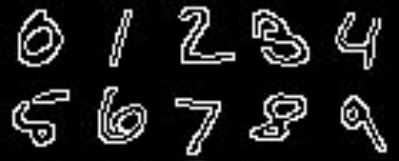
\includegraphics[width=0.25\textwidth]{figures/canny}
			\caption{Muestra de imagen con filtro Canny}
			\label{fig.canny}
		\end{center}
	\end{figure}
	
	\item[Filtro Laplaciano] \hfill 
	\vspace{10pt}
	\\
	El operador laplaciano es un segundo operador derivado que se utiliza con frecuencia en la detección de bordes. \cite{4135681}
	\item[Filtro de Sobel] \hfill 
	\vspace{10pt}
	\\
\end{description}

\subsection{Número de neuronas}

\subsection{Dropout}

\section{Experimentos}



